\documentclass[tikz,border=1mm]{standalone}

\usepackage{amsmath}
\usepackage{graphicx}
\renewcommand\familydefault{\sfdefault} 
\usepackage[T1]{fontenc}

\usetikzlibrary{arrows,shapes,calc,math,decorations.fractals,patterns,backgrounds,decorations.markings}
\tikzset{every picture/.style={/utils/exec={\sffamily}}}
\tikzset{point/.style={fill,circle,inner sep=1.5pt}}
\tikzset{vel/.style={-triangle 45,blue!50!black,line width=1pt}}
\tikzset{acc/.style={-triangle 45,red,line width=1pt}}
\tikzset{myarrow/.style={decoration={markings,mark=at position 1 with %
    {\arrow[scale=3,>=stealth]{>}}},postaction={decorate}}}

\begin{document}

% agent
\newcommand{\agent}[4]{
    \draw [fill=#3,line width=1pt] ($#1+({#4*cos(#2)}, {#4*sin(#2)})$) 
        -- ($#1+({-0.5*#4*cos(#2)-0.5*#4*sin(#2)}, {-0.5*#4*sin(#2)+0.5*#4*cos(#2)})$)
        -- ($#1+({-0.5*#4*cos(#2)+0.5*#4*sin(#2)}, {-0.5*#4*sin(#2)-0.5*#4*cos(#2)})$)
        -- cycle;
}

% field
% \begin{tikzpicture}
%     \draw (0, 0) rectangle ++(6, 4);
%     \draw [latex'-latex'] (0, -0.5) -- ++(6, 0) node [pos=0.5,fill=white] {width};
%     \draw [latex'-latex'] (6.3,0) -- ++(0, 4) node [pos=0.5,fill=white,rotate=90] {height};
%     \coordinate (p1) at (2,1);
%     \coordinate (p2) at (5,1);
%     \coordinate (p3) at (4.5,2.75);
%     \coordinate (p4) at (1.5,3);
%     \agent{(p1)}{45}{blue!10}{0.5};
%     \agent{(p2)}{80}{blue!10}{0.5};
%     \agent{(p3)}{30}{blue!10}{0.5};
%     \agent{(p4)}{340}{blue!10}{0.5};
%     \node [point] at (p1) (p1) {};
%     \draw [help lines,dashed] (-0.4,1) -- (2,1) -- (2, -0.4);
%     \draw [latex'-latex'] (0,-0.25) -- ++(2,0) node [pos=0.5,fill=white] {$x$};
%     \draw [latex'-latex'] (-0.25,0) -- ++(0,1) node [pos=0.5,fill=white] {$y$};
%     \draw [-triangle 45, blue!50!black,thick] ($(p1)+(45:0.5)$) -- ($(p1)+(1,1)$);
%     \draw [latex'-latex',help lines] ($(p1)$) -- ++(1,0) node [pos=0.6,below,black] {$v_x$};
%     \draw [latex'-latex',help lines] ($(p1)+(1.05,0)$) -- ++(0,1) node [pos=0.5,right,black] {$v_y$};
% \end{tikzpicture}

% agent
% \tikzmath{\v=2.5;\a=20;\p=45;\r=2.5;}
% \begin{tikzpicture}
%     \coordinate (p1) at (\p:\r);
%     \coordinate (p2) at ($(p1)+(\a:\v)$);
%     \coordinate (p3) at ($(p2)+(\a:\v)$);
%     \node [point] at (p1) (p1) {};
%     \draw [vel] ($(p1)$) -- ++(\a:\v) node [pos=0.6,above,rotate=\a] {velocity};
%     \agent{(p1)}{\a}{blue!10}{1}
%     \draw [-stealth'] (0, 0) -- ++(5, 0);
%     \draw [-stealth'] (0, 0) -- ++(0, 3);
%     \draw [-triangle 45] (0, 0) -- (p1) node [pos=0.5,below,rotate=\p] {position};
%     \draw [latex'-latex'] (0,-0.2) -- node [fill=white] {$x$} ++({\r*cos(\p)},0);
%     \draw [latex'-latex'] (-0.25,0) -- node [fill=white] {$y$} ++(0,{\r*sin(\p)});
%     \draw [latex'-latex'] (p1) -- node [fill=white] {$v_x$} ++({\v*cos(\a)}, 0);
%     \draw [latex'-latex'] ($(p1)+({\v*cos(\a)+0.1},0)$) -- node [fill=white] {$v_y$} ++(0, {\v*sin(\a)});
%     \node [point] at (p1) {};
% \end{tikzpicture}

% movement
% \tikzmath{\v=3;\a=10;}
% \begin{tikzpicture}[auto]
%     \coordinate (p1) at (0, 0);
%     \coordinate (p2) at ($(p1)+(\a:\v)$);
%     \coordinate (p3) at ($(p2)+(\a:\v)$);
%     \draw [vel] (p1) -- ++(\a:2.5) node [pos=0.6,below,rotate=\a] {velocity};
%     \draw [vel] (p2) -- ++(\a:2.5) node [pos=0.6,below,rotate=\a] {velocity};
%     \draw [vel] (p3) -- ++(\a:2.5) node [pos=0.6,below,rotate=\a] {velocity};
%     \agent{(p1)}{\a}{blue!10}{1}
%     \agent{(p2)}{\a}{blue!10}{1}
%     \agent{(p3)}{\a}{blue!10}{1}
%     \node at (p1) {$\mathbf{p}_1$};
%     \node at (p2) {$\mathbf{p}_2$};
%     \node at (p3) {$\mathbf{p}_3$};
% \end{tikzpicture}

% steering vectors
% \begin{tikzpicture}
%     \coordinate (p1) at (0, 0);
%     \coordinate (p2) at (80:2.5);
%     \coordinate (p3) at (180:2);
%     \coordinate (p4) at (30:1);
%     \agent{(p1)}{90}{blue!10}{1}
%     \draw [vel, green!75!black] (p1) -- (p2) node [right] {steering 1};
%     \draw [vel, green!75!black] (p1) -- (p3) node [left] {steering 2};
%     \draw [vel, green!75!black] (p1) -- (p4) node [right] {steering 3};
%     \draw [acc] (p1) -- ($(p2)+(p3)+(p4)$) node [left] {acceleration};
%     \agent{(p1)}{90}{blue!10}{1}
% \end{tikzpicture}

% target
\tikzmath{\v0=90; \s=2; \a1=0; \ta=15; \td=5; \dv=20; \da=20;
    \v1=\v0-\dv; \v2=\v1-\dv; \v3=\v2-\dv; \v4=\v3-\dv; \v5=\v4-\dv; \v6=\v5-\dv;
    \a2=\a1-\da; \a3=\a2-\da; \a4=\a3-\da; \a5=\a4-\da; \a6=\a5-\da;}
% \begin{tikzpicture}[auto]
%     \coordinate (p0) at (0, 0);
%     \coordinate (p1) at ($(p0)+(\v1:\s)$);
%     \coordinate (p2) at ($(p1)+(\v2:\s)$);
%     \coordinate (p3) at ($(p2)+(\v3:\s)$);
%     \coordinate (p4) at ($(p3)+(\v4:\s)$);
%     \draw (\ta:\td) coordinate (target) circle (0.2);
%     \draw [vel] ($(p0)+(\v0:1)$) -- ($(p0)+(\v0:\s)$) node [above] {velocity};
%     \draw [vel,green!75!black] (p0) -- (target) node [pos=0.5,above,rotate=\ta] {steering = target - position};
%     \draw ($(target)+(0,-0.4)$) -- ++(0,0.8) node [pos=0,below] {target};
%     \draw ($(target)+(-0.4,0)$) -- ++(0.8,0);
%     \agent{(p0)}{\v0}{blue!10}{1}
% \end{tikzpicture}

% \begin{tikzpicture}[auto]
%     \coordinate (p0) at (0, 0);
%     \coordinate (p1) at ($(p0)+(\v1:\s)$);
%     \coordinate (p2) at ($(p1)+(\v2:\s)$);
%     \coordinate (p3) at ($(p2)+(\v3:\s)$);
%     \coordinate (p4) at ($(p3)+(\v4:\s)$);
%     \draw (\ta:\td) coordinate (target) circle (0.2);
%     \draw [vel] (p0) -- (70:\s) node [above right,text width=4cm] {new velocity $=$ velocity $+$ acceleration};
%     \draw [vel,gray] ($(p0)+(\v0:1)$) -- ($(p0)+(\v0:\s)$) node [above] {velocity};    \draw [acc] (p0) -- ($(p0)!1.5cm!(target)$) node [pos=1,below,rotate=\ta] {acceleration};
%     \draw [vel,green!75!black] ($(p0)!1.5cm!(target)$) -- (target) node [pos=0.5,above,rotate=\ta] {steering};
%     \draw ($(target)+(0,-0.4)$) -- ++(0,0.8) node [pos=0,below] {target};
%     \draw ($(target)+(-0.4,0)$) -- ++(0.8,0);
%     \agent{(p0)}{\v0}{gray!10}{1}
%     \agent{(p0)}{70}{blue!10}{1}
% \end{tikzpicture}

% \begin{tikzpicture}[auto]
%     \coordinate (p0) at (0, 0);
%     \coordinate (p1) at ($(p0)+(\v1:\s)$);
%     \coordinate (p2) at ($(p1)+(\v2:\s)$);
%     \coordinate (p3) at ($(p2)+(\v3:\s)$);
%     \coordinate (p4) at ($(p3)+(\v4:\s)$);
%     \coordinate (p5) at ($(p4)+(\v5:\s)$);
%     \draw (9.35,3.4) coordinate (target) circle (0.2);
%     \draw ($(target)+(0,-0.4)$) -- ++(0,0.8) node [pos=0,below] {target};
%     \draw ($(target)+(-0.4,0)$) -- ++(0.8,0);
%     % \agent{(p0)}{\v0}{gray!10}{1}
%     % \agent{(p1)}{\v1}{gray!10}{1}
%     % \agent{(p2)}{\v2}{gray!10}{1}
%     % \agent{(p3)}{\v3}{gray!10}{1}
%     % \agent{(p4)}{\v4}{gray!10}{1}
%     % \agent{(p5)}{\v5}{gray!10}{1}
%     \draw [acc] (p0) -- ($(p0)!1.5cm!(target)$);
%     \draw [acc] (p1) -- ($(p1)!1.5cm!(target)$);
%     \draw [acc] (p2) -- ($(p2)!1.5cm!(target)$);
%     \draw [acc] (p3) -- ($(p3)!1.5cm!(target)$);
%     \draw [acc] (p4) -- ($(p4)!1.5cm!(target)$);
%     \draw [acc] (p5) -- ($(p4)!1.5cm!(target)$);
%     % \draw [vel,gray,opacity=1] ($(p0)+(\v0:1)$) -- ($(p0)+(\v0:\s)$);
%     % \draw [vel,gray,opacity=1] ($(p1)+(\v1:1)$) -- ($(p1)+(\v1:\s)$);
%     % \draw [vel,gray,opacity=1] ($(p2)+(\v2:1)$) -- ($(p2)+(\v2:\s)$);
%     % \draw [vel,gray,opacity=1] ($(p3)+(\v3:1)$) -- ($(p3)+(\v3:\s)$);
%     % \draw [vel,gray,opacity=1] ($(p4)+(\v4:1)$) -- ($(p4)+(\v4:\s)$);
%     % \draw [vel,gray,opacity=1] ($(p5)+(\v5:1)$) -- ($(p5)+(\v5:\s)$);
%     \agent{(p0)}{\v1}{blue!10}{1}
%     \agent{(p1)}{\v2}{blue!10}{1}
%     \agent{(p2)}{\v3}{blue!10}{1}
%     \agent{(p3)}{\v4}{blue!10}{1}
%     \agent{(p4)}{\v5}{blue!10}{1}
%     \agent{(p5)}{\v6}{blue!10}{1}
%     \draw [vel] ($(p0)+(\v1:1)$) -- ($(p0)+(\v1:\s)$);
%     \draw [vel] ($(p1)+(\v2:1)$) -- ($(p1)+(\v2:\s)$);
%     \draw [vel] ($(p2)+(\v3:1)$) -- ($(p2)+(\v3:\s)$);
%     \draw [vel] ($(p3)+(\v4:1)$) -- ($(p3)+(\v4:\s)$);
%     \draw [vel] ($(p4)+(\v5:1)$) -- ($(p4)+(\v5:\s)$);
%     \draw [vel] ($(p5)+(\v6:1)$) -- ($(p5)+(\v6:\s)$);
% \end{tikzpicture}

% random walk
% \tikzmath{\a=60; \d=4; \t1=90;\t2=120;}

% \begin{tikzpicture}
%     \coordinate (p1) at (0, 0);
%     \coordinate (target) at (\t2:\d);
%     \fill [help lines, fill=green!10] (0, 0) -- ({\a + \t1}:\d) arc ({\a+\t1}:{\a-\t1}:\d) -- cycle;
%     \draw [help lines, dashed] (0, 0) -- (\a:\d);
%     \draw [latex'-latex',help lines] (\a:\d) arc (\a:{\a-\t1}:\d) node [pos=0.5,right,black] {$\textsf{agent angle} - \dfrac{\pi}{2}$};
%     \draw [latex'-latex',help lines] (\a:\d) arc (\a:{\a+\t1}:\d) node [pos=0.4,above,black] {$\textsf{agent angle} - \dfrac{\pi}{2}$};
%     \draw [help lines] (0, 0) -- (0:\d);
%     \draw [fill=white] (target) circle (0.2);
%     \draw ($(target)+(-0.4,0)$) -- ++(0.8,0);
%     \draw ($(target)+(0,-0.4)$) -- ++(0,0.8) node [left] {target};
%     \draw [vel] ($(p1)+(\a:1)$) -- ++(\a:1);
%     \draw [vel,green!75!black] (p1) -- (target);
%     \agent{(p1)}{60}{blue!10}{1}
%     \draw [latex'-,help lines] (\a:1.2) arc (\a:0:1.2) node [pos=0.5,right,black,text width=1cm] {agent angle};
%     \draw [latex'-,help lines] (\t2:2.5) arc (\t2:0:2.5) node [pos=0.3,above right,black,text width=1cm] {target angle};
%     \draw [-latex',help lines] (\a:1.2) arc (\a:\t2:1.2) node [pos=0.5,above,black,text width=1cm] {random angle};
%     % \draw [-latex', help lines] (\a:\d) arc (\a:{\a+\t}:\d) node [pos=0.5,above] {$-\frac{1}{2}\pi$};
%     % \draw [latex'-latex', help lines] (\a:{0.6*\d}) arc (\a:{\a+\t1}:{0.6*\d}) node [pos=0.5,above] {$\frac{1}{2}\pi$};
% \end{tikzpicture}

% edges
% \tikzmath{\a1=315;\a2=340;\a3=0;\a4=20;\a5=45;\a6=45;\l=2.5;}
% \begin{tikzpicture}[auto]
%     \coordinate (p1) at (1, 3.5);
%     \coordinate (p2) at ($(p1)+(\a1:\l)$);
%     \coordinate (p3) at ($(p2)+(\a2:\l)$);
%     \coordinate (p4) at ($(p3)+(\a3:\l)$);
%     \coordinate (p5) at ($(p4)+(\a4:\l)$);
%     \coordinate (p6) at ($(p5)+(\a5:\l)$);
%     \coordinate (p7) at ($(p2)+(\a1:\l)$);
%     \coordinate (p8) at ($(p7)+(\a1:\l)$);
%     \fill [pattern=north east lines] (0, 0) rectangle ++(14, -0.25);
%     \draw [line width=1pt] (0, 0) -- ++(14, 0);
%     \node [below] at (8,-0.25) {edge}; 
%     \fill [green!10] (0, 0) rectangle ++(14,3);
%     \tikzmath{\cos=cos(\a1);\sin=sin(\a1);}
%     \agent{(p2)}{\a1}{gray!10}{1}
%     \agent{(p7)}{\a1}{gray!10}{1}
%     \agent{(p8)}{\a1}{gray!10}{1}
%     \draw [vel,gray,opacity=1] ($(p2)+(\a1:1)$) -- ++(\a1:{\l-1});
%     \draw [vel,gray,opacity=1] ($(p7)+(\a1:1)$) -- ++(\a1:{\l-1});
%     \draw [acc] (p2) -- ++(90:1.5);
%     \draw [acc] (p3) -- ++(90:3);
%     \draw [acc] (p4) -- ++(90:3);
%     \draw [acc] (p5) -- ++(90:1.5);
%     \agent{(p1)}{\a1}{blue!10}{1}
%     \agent{(p2)}{\a2}{blue!10}{1}
%     \agent{(p3)}{\a3}{blue!10}{1}
%     \agent{(p4)}{\a4}{blue!10}{1}
%     \agent{(p5)}{\a5}{blue!10}{1}
%     \agent{(p6)}{\a6}{blue!10}{1}
%     \draw [vel] ($(p1)+(\a1:1)$) -- ++(\a1:{\l-1});
%     \draw [vel] ($(p2)+(\a2:1)$) -- ++(\a2:{\l-1});
%     \draw [vel] ($(p3)+(\a3:1)$) -- ++(\a3:{\l-1});
%     \draw [vel] ($(p4)+(\a4:1)$) -- ++(\a4:{\l-1});
%     \draw [vel] ($(p5)+(\a5:1)$) -- ++(\a5:{\l-1});
%     \draw [stealth'-stealth'] (13,0) -- ++(0,3) node [pos=0.5,left] {buffer};
% \end{tikzpicture}

% neighbouring agents
% \begin{tikzpicture}
%     \coordinate (p1) at (0, 0);
%     \coordinate (p2) at (-2.5, 1.25);
%     \coordinate (p3) at (2, 3);
%     \coordinate (p4) at (-3,-3);
%     \coordinate (p5) at (-6,3);
%     \coordinate (p6) at (6,-3);
%     \draw [line width=1pt,fill=green!10] circle (5cm);
%     \agent{(p1)}{90}{green!75!black}{1}
%     \agent{(p2)}{110}{blue!10}{1}
%     \agent{(p3)}{45}{blue!10}{1}
%     \agent{(p4)}{120}{blue!10}{1}
%     \agent{(p5)}{70}{gray!20}{1}
%     \agent{(p6)}{100}{gray!20}{1}
%     % \draw [latex'-latex'] (0,0) -- (0:5) node [pos=0.5,below] {detection radius};
% \end{tikzpicture}

% separation
% \tikzmath{\a1=90;\a2=100;\a3=80;\a4=110;\l=3;}
% \begin{tikzpicture}[background rectangle/.style={fill=green!10}, show background rectangle]
%     \coordinate (p1) at (0, 0);
%     \coordinate (p2) at (-1.5, 1.25);
%     \coordinate (p3) at (2, 3);
%     \coordinate (p4) at (-3,-3);
%     \coordinate (p5) at (-6,3);
%     \coordinate (p6) at (6,-3);
%     \draw [line width=1pt,fill=red!10] circle (5cm);
%     \draw (p2) -- (p1) (p3) -- (p1) (p4) -- (p1);
%     \draw [-triangle 45,line width=2pt,red] (p1) -- ++(330:3);
%     \agent{(p1)}{\a1}{green!75!black}{1}
%     \agent{(p2)}{\a2}{red!40}{1}
%     \agent{(p3)}{\a3}{red!40}{1}
%     \agent{(p4)}{\a4}{red!40}{1}
%     \agent{(p5)}{\a4}{blue!10}{1}
%     \agent{(p6)}{\a3}{blue!10}{1}
%     % \draw [latex'-latex'] (p1) -- ++(0:5) node [pos=0.5,below] {separation radius};
% \end{tikzpicture}

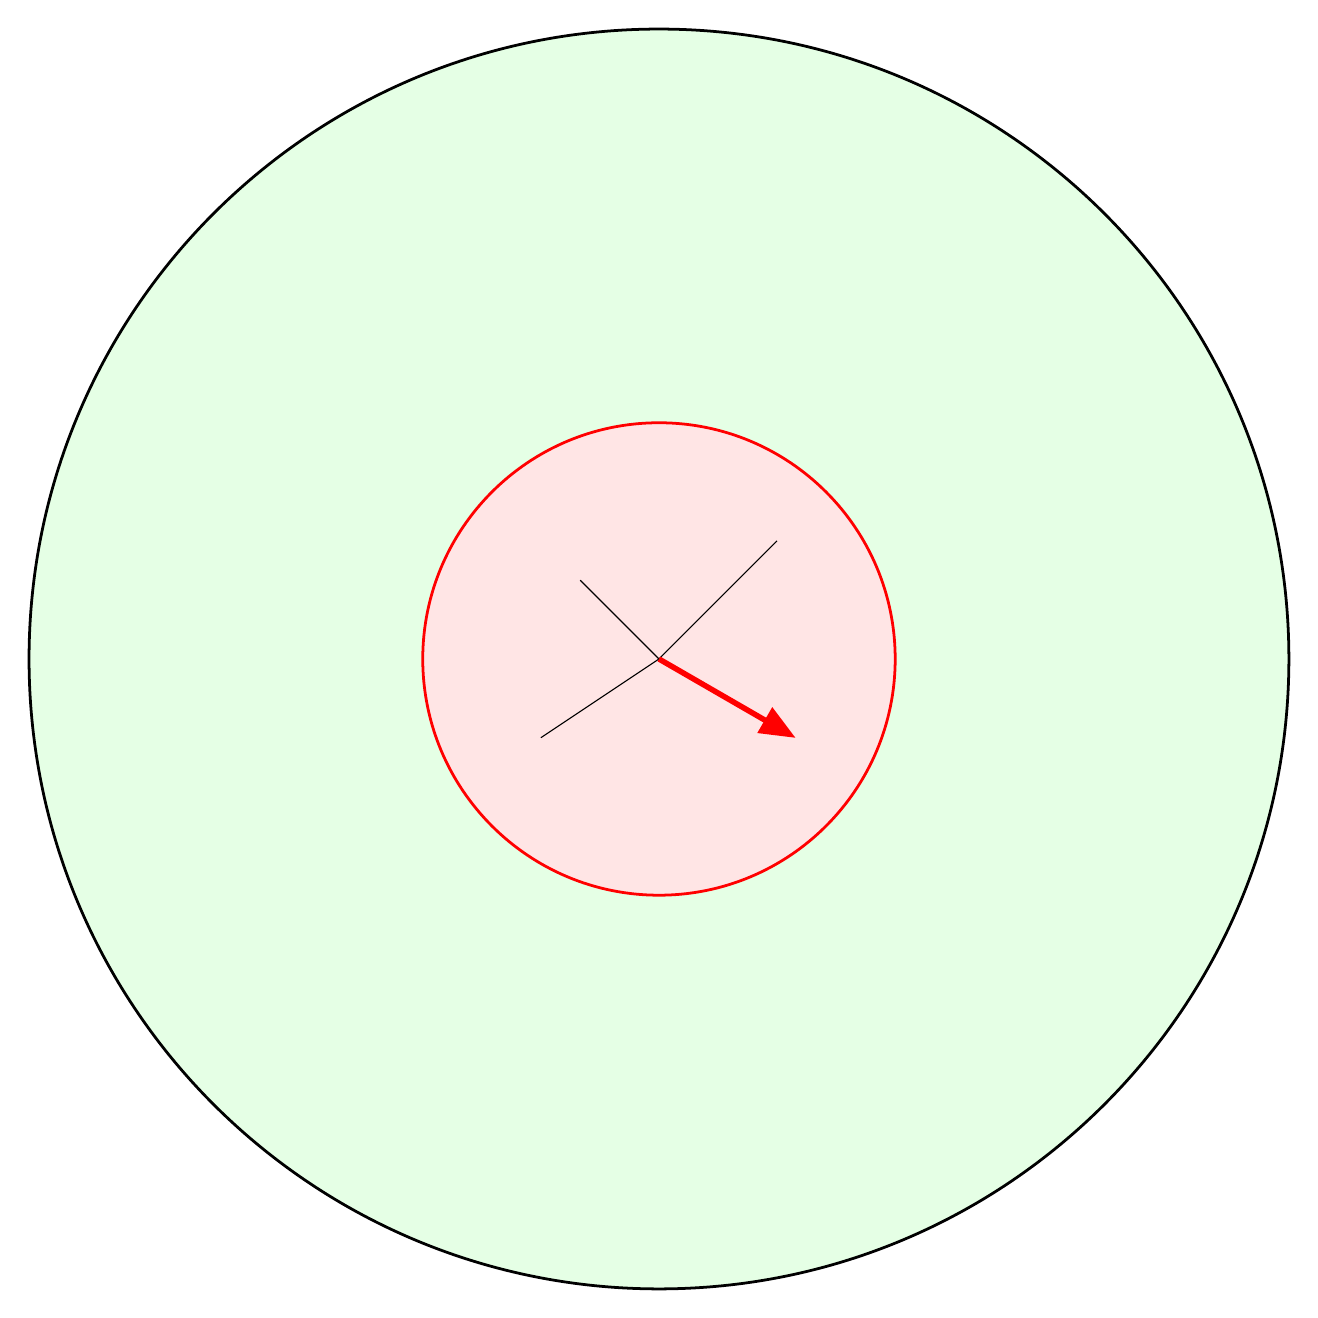
\begin{tikzpicture}
    \draw [line width=1pt, fill=green!10] circle (8cm);
    \draw [red, line width=1pt, fill=red!10] circle (3cm);
    \draw (0, 0) -- (-1,1) (0, 0) -- (1.5,1.5) (0, 0) -- (-1.5, -1);
    \draw [acc,line width=2pt] (0, 0) -- (-30: 2);
    \agent{(0,0)}{90}{green!75!black}{0.5}
    \agent{(-1,1)}{100}{red!40}{0.5}
    \agent{(1.5,1.5)}{80}{red!40}{0.5}
    \agent{(-1.5,-1)}{100}{red!40}{0.5}
    \agent{(-3,4)}{100}{blue!10}{0.5}
    \agent{(-5,0)}{95}{blue!10}{0.5}
    \agent{(-3,-5)}{100}{blue!10}{0.5}
\end{tikzpicture}

% alignment
% \tikzmath{\a1=90;\a2=100;\a3=80;\a4=130;\a5=120;\a6=90;\l=3;
%     \a7 = (\a2+\a3+\a4+\a5+\a6) / 5;}
% \begin{tikzpicture}
%     \coordinate (p1) at (0, 0);
%     \coordinate (p2) at (-2, 2);
%     \coordinate (p3) at (2, 2.5);
%     \coordinate (p4) at (-2,-3);
%     \coordinate (p5) at (-3,0);
%     \coordinate (p6) at (2,-2.5);
%     \draw [line width=1pt,fill=green!10] circle (5cm);

%     \draw [-triangle 45,gray] (p1) -- ++(\a1:2);
%     \draw [vel] (p2) -- ++(\a2:2);
%     \draw [vel] (p3) -- ++(\a3:2);
%     \draw [vel] (p4) -- ++(\a4:2);
%     \draw [vel] (p5) -- ++(\a5:2);
%     \draw [vel] (p6) -- ++(\a6:2);
%     \draw [vel] (p1) -- ++(\a7:2);
%     \draw [vel,line width=2pt,red] (p1) -- ++(190:1.5);
%     \draw [fill=gray!10,thick] ($(p1)+({cos(\a1)}, {sin(\a1)})$) 
%         -- ($(p1)+({-0.5*cos(\a1)-0.5*sin(\a1)}, {-0.5*sin(\a1)+0.5*cos(\a1)})$)
%         -- ($(p1)+({-0.5*cos(\a1)+0.5*sin(\a1)}, {-0.5*sin(\a1)-0.5*cos(\a1)})$) -- cycle;
%     \draw [fill=blue!10,thick] ($(p2)+({cos(\a2)}, {sin(\a2)})$) 
%         -- ($(p2)+({-0.5*cos(\a2)-0.5*sin(\a2)}, {-0.5*sin(\a2)+0.5*cos(\a2)})$)
%         -- ($(p2)+({-0.5*cos(\a2)+0.5*sin(\a2)}, {-0.5*sin(\a2)-0.5*cos(\a2)})$) -- cycle;
%     \draw [fill=blue!10,thick] ($(p3)+({cos(\a3)}, {sin(\a3)})$) 
%         -- ($(p3)+({-0.5*cos(\a3)-0.5*sin(\a3)}, {-0.5*sin(\a3)+0.5*cos(\a3)})$)
%         -- ($(p3)+({-0.5*cos(\a3)+0.5*sin(\a3)}, {-0.5*sin(\a3)-0.5*cos(\a3)})$) -- cycle;
%     \draw [fill=blue!10,thick] ($(p4)+({cos(\a4)}, {sin(\a4)})$) 
%         -- ($(p4)+({-0.5*cos(\a4)-0.5*sin(\a4)}, {-0.5*sin(\a4)+0.5*cos(\a4)})$)
%         -- ($(p4)+({-0.5*cos(\a4)+0.5*sin(\a4)}, {-0.5*sin(\a4)-0.5*cos(\a4)})$) -- cycle;
%     \draw [fill=blue!10,thick] ($(p5)+({cos(\a5)}, {sin(\a5)})$) 
%         -- ($(p5)+({-0.5*cos(\a5)-0.5*sin(\a5)}, {-0.5*sin(\a5)+0.5*cos(\a5)})$)
%         -- ($(p5)+({-0.5*cos(\a5)+0.5*sin(\a5)}, {-0.5*sin(\a5)-0.5*cos(\a5)})$) -- cycle;
%     \draw [fill=blue!10,thick] ($(p6)+({cos(\a6)}, {sin(\a6)})$) 
%         -- ($(p6)+({-0.5*cos(\a6)-0.5*sin(\a6)}, {-0.5*sin(\a6)+0.5*cos(\a6)})$)
%         -- ($(p6)+({-0.5*cos(\a6)+0.5*sin(\a6)}, {-0.5*sin(\a6)-0.5*cos(\a6)})$) -- cycle;
%     \draw [fill=green!75!black,thick] ($(p1)+({cos(\a7)}, {sin(\a7)})$) 
%         -- ($(p1)+({-0.5*cos(\a7)-0.5*sin(\a7)}, {-0.5*sin(\a7)+0.5*cos(\a7)})$)
%         -- ($(p1)+({-0.5*cos(\a7)+0.5*sin(\a7)}, {-0.5*sin(\a7)-0.5*cos(\a7)})$) -- cycle;
% \end{tikzpicture}

% cohesion
% \tikzmath{\a1=90;\a2=100;\a3=80;\a4=80;\a5=120;\a6=110;\l=3;
%     \a7 = (\a2+\a3+\a4+\a5+\a6) / 5;}
% \begin{tikzpicture}[semithick]
%     \coordinate (p1) at (0, 0);
%     \coordinate (p2) at (-2, 2);
%     \coordinate (p3) at (-6, 2.5);
%     \coordinate (p4) at (-1.5,-3);
%     \coordinate (p5) at (-4,0);
%     \coordinate (p6) at (-6,-2.5);
%     \draw [line width=1pt,fill=green!10] circle (5cm);
%     \node [circle,fill,inner sep=2pt] at ($0.33*(p2)+0.33*(p4)+0.33*(p5)$) (c) {} ;
%     \draw [line width=1pt] (p2) -- (c) (p4) -- (c) (p5) -- (c);
%     \draw [-triangle 45,line width=2pt,red] (p1) -- (c);
%     \agent{(p1)}{\a1}{green!75!black}{1}
%     \agent{(p2)}{\a2}{blue!10}{1}
%     \agent{(p3)}{\a3}{gray!10}{1}
%     \agent{(p4)}{\a4}{blue!10}{1}
%     \agent{(p5)}{\a4}{blue!10}{1}
%     \agent{(p6)}{\a3}{gray!10}{1}
% \end{tikzpicture}

\end{document}